\documentclass{article}
\usepackage{blindtext}
\usepackage{multirow}
\usepackage{threeparttable}
\usepackage{booktabs}
\usepackage{graphicx}

\begin{document}
\title{The Science of Learning LaTex}
\author{Tobias Klöpper \thanks{Many thanks especially to Marco, his company and the delicious beer he provides} \\
\normalsize University of Zurich
\and Marco Barcellos \thanks{Many thanks to all the beers that have allowed me to go on}\\
\normalsize University of Minsk}
\date{13th of October 2021}
\maketitle
\begin{abstract}
This paper discusses the Science of Learning LaTeX. In particular it provides valuable insights into the difficult Learning Process of Tobias Klöpper who is trying to make this stuff work.
\end{abstract}
\section{Introduction}
\Blindtext
\newpage
\section{Figures and Tables}
The following Table \ref{table:1} shows a list of beers and my assessment of them.
\begin{table}[h!]
\begin{tabular}{ |p{3cm}||p{3cm}|p{3cm}|p{3cm}|  }
 \hline
 \multicolumn{4}{|c|}{Beer Ratings} \\
 \hline
 Beer Name & Country of Origin &Type of beer&Rating\\
 \hline
 Krombacher   & Germany    & Pils &   6/10\\
 Oettinger&   Germany  & Export   &10/10\\
 Feldschlösschen &Switzerland & Lager &  5/10\\
 Heineken    &Netherlands & Lager &  5/10\\
 Pilsner Urquell&   Czech Republic  & Pils & 7/10\\
 Arany Àszok& Hungary  & Lager   & 2/10\\
 Dreher& Hungary  & Pils & 5/10\\
 \hline
 \end{tabular}
 \caption{Own assessment of beers}
 \label{table:1}
\end{table}

\par
Lets test another package with Table \ref{table:2}
\begin{table}[h]
\begin{center}
\begin{threeparttable}
\begin{tabular}{c c c c}
    \toprule
    \textbf{Beer Name} & \textbf{Country of Origin} & \textbf{Type of Beer} & \textbf{Rating} \\ 
    \midrule
      Oettinger Export\tnote{1}   & Germany & Pils & 10/10 \\
      Oettinger Pils\tnote{2}   & Germany & Export & 2/10 \\ 
      \bottomrule
\end{tabular}
\begin{tablenotes}
\item[1] actually quite pleasant, even cheaply attainable in Kiosks for about 1€; \item[2] only consume ice cold, tastes way better after you already had a couple of beers
\end{tablenotes}
\end{threeparttable}
\end{center}
\caption{Beer Ratings with new packages}{}
\label{table:2}
\end{table}

\par

The following figure shows a nice beer \ref{figure:1}
      \begin{figure}[htb]\center 
        \begin{tabular}{c}
          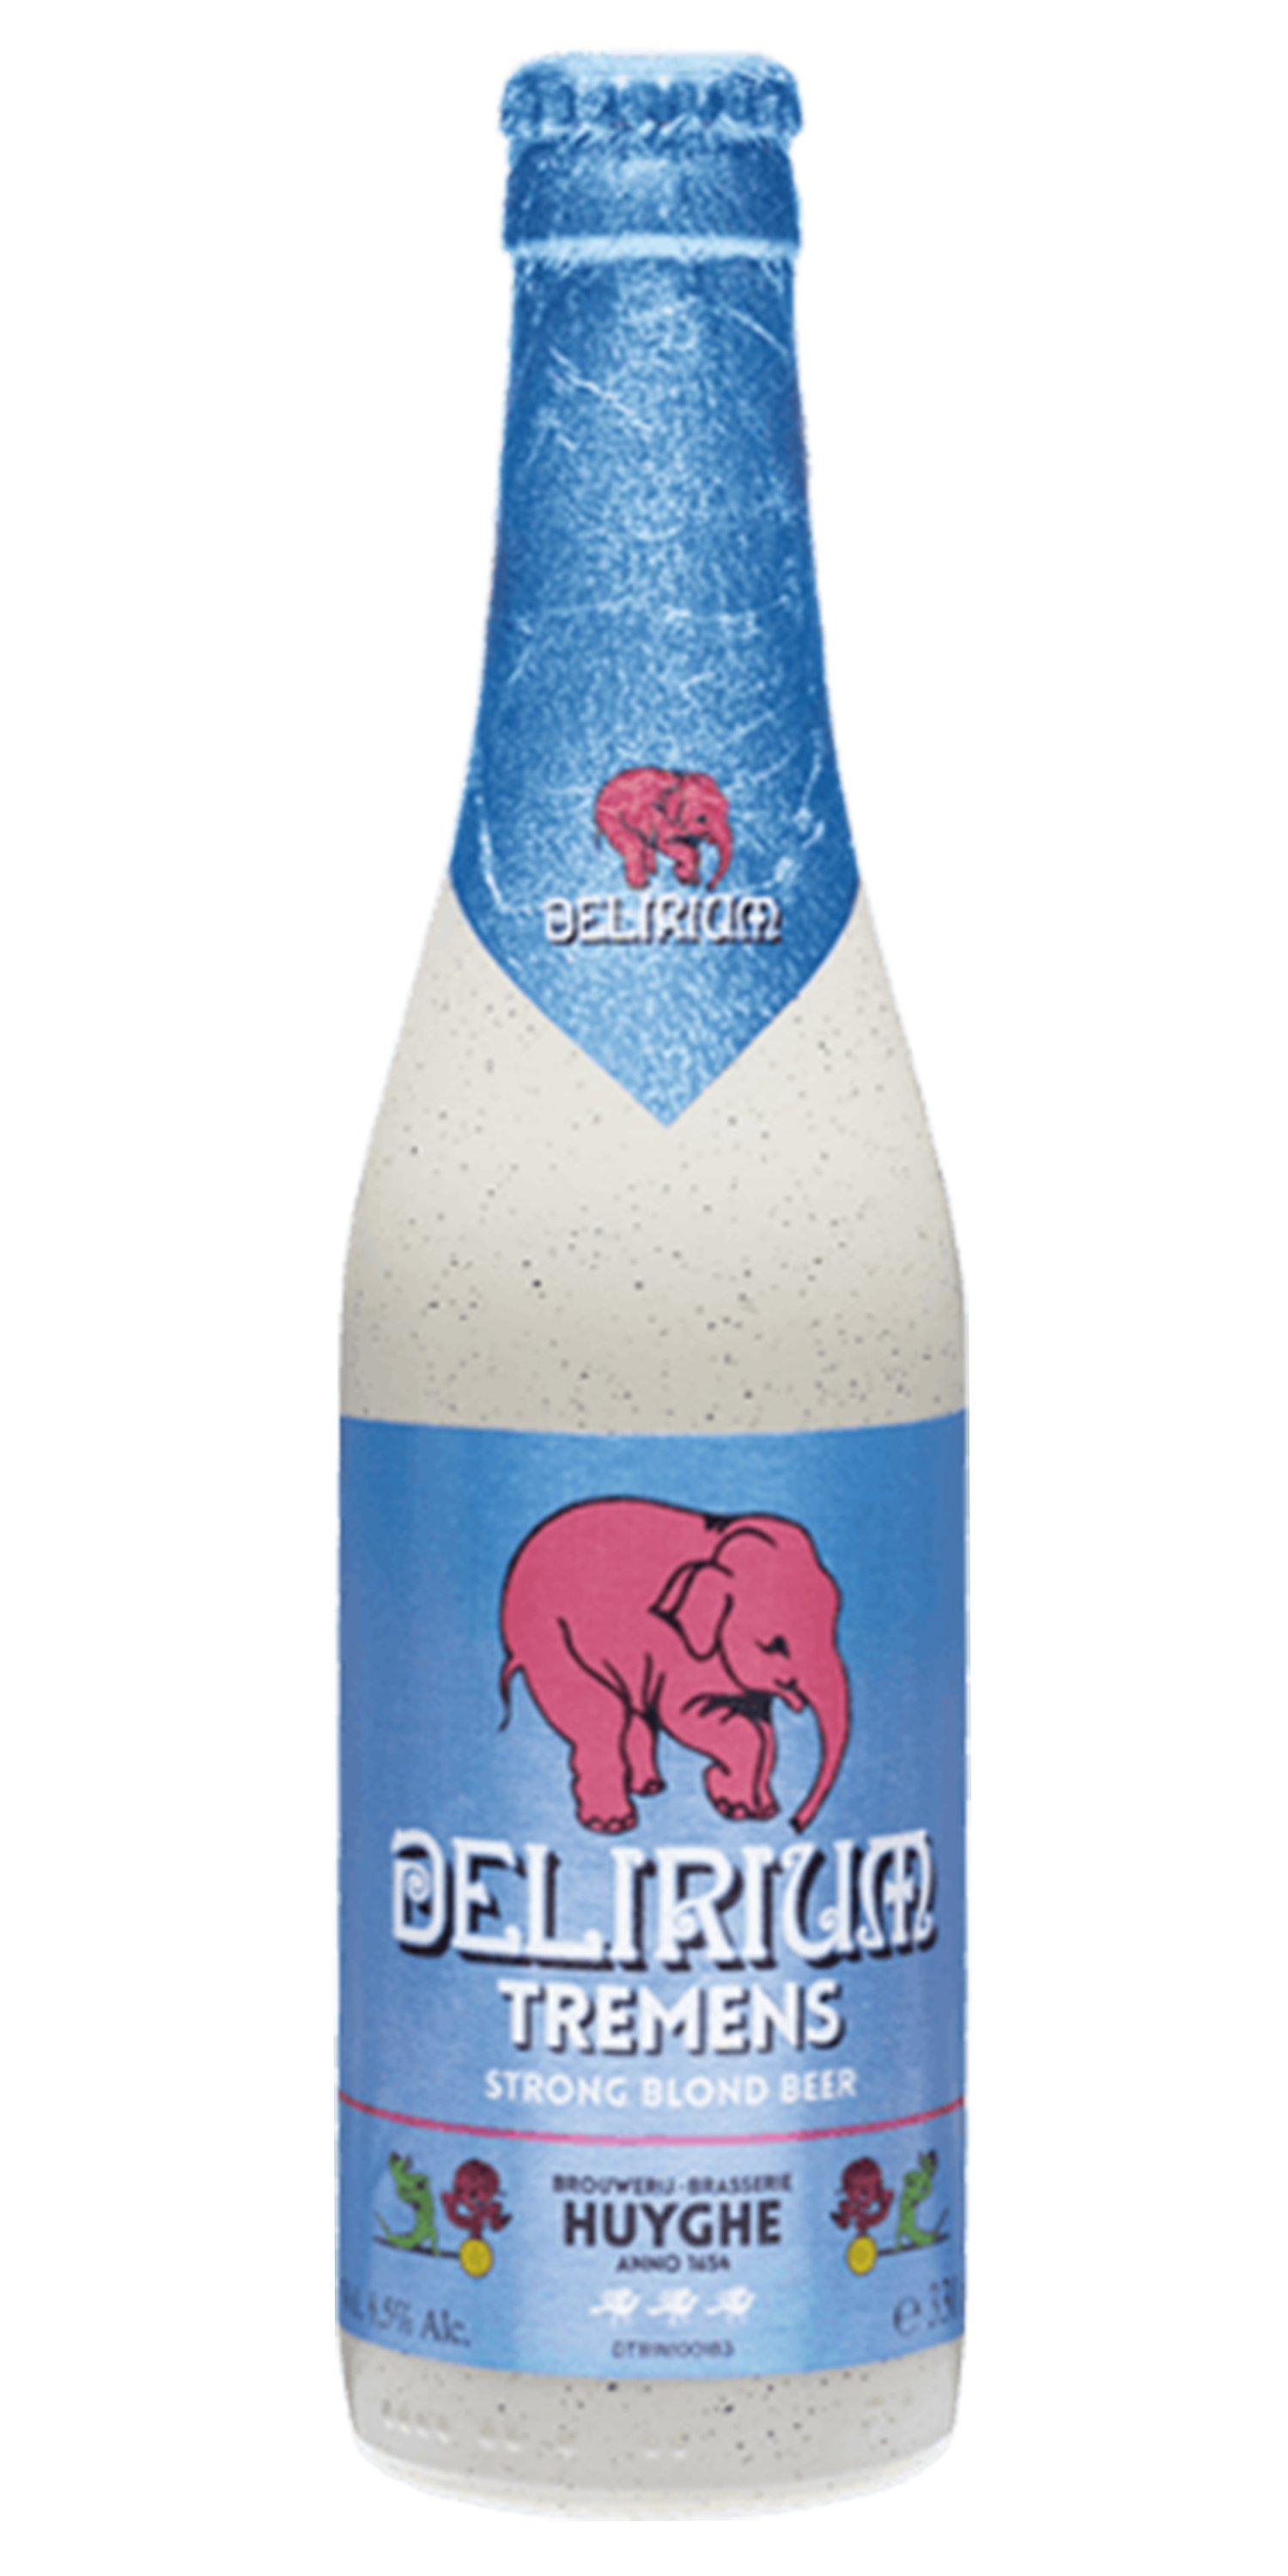
\includegraphics[width=7cm]{important_figure.jpg}
        \end{tabular}
        \caption{\footnotesize BEER}
        \label{figure:1}
      \end{figure}

\end{document}
